\documentclass{beamer}
\usepackage{amsmath,mathrsfs,amsfonts,amssymb}
\usepackage{graphicx, epsfig}
\usepackage{subfig}
\usepackage{floatflt}
\usepackage{epic,ecltree}
\usepackage{mathtext}
\usepackage{fancybox}
\usepackage{fancyhdr}
\usepackage{enumerate}
\usepackage{epstopdf}
\usepackage{animate}
\usepackage{caption}
\usepackage{cite}
\usepackage{natbib}
\setbeamercovered{transparent}
\setbeamertemplate{caption}{\raggedright\insertcaption\par}

\usetheme{Warsaw}
\usecolortheme{sidebartab}

\title[\hbox to 56mm{Bipedal robot locomotion control\hfill\insertframenumber\,/\,\inserttotalframenumber}]
            {Development and implementation dynamic balance algorithms for bipedal robot locomotion}
\author{Usvyastov Mikhail}
\institute[Innopolis]{Innopolis University\\
    Final presentation\\
    Supervisor: Evgeni Magid
}

\date{\normalsize \today}

\begin{document}
	% Creates title page of slide show using above information
	\begin{frame}
	  \titlepage
	\end{frame}

%%%%%%%%%%%%%%%%%%%%%%%%%%%%%%%%%%%%%%%%%%%%%%%%%%%%%%%%%%%%%%%%%%%%%%%%%%%%%%%%%%%%%%%%%%%%%%%%%%%%%

	\begin{frame}
		\frametitle{Outline}
		\begin{itemize}
			\item Introduction and Motivation
			\item Problem Overview
			\item Related work
			\item Theoretical aspects of bipedal robots control
			\item Implementation and evaluation
			\item Future work
			\item Summary
		\end{itemize}
	\end{frame}

%%%%%%%%%%%%%%%%%%%%%%%%%%%%%%%%%%%%%%%%%%%%%%%%%%%%%%%%%%%%%%%%%%%%%%%%%%%%%%%%%%%%%%%%%%%%%%%%%%%%%

	\begin{frame}
		\frametitle{Introduction and Motivation: the development of robotics in minds}
		\centering
		Trends in robotics are near to be developed.
		
		\begin{figure}[h!]
			\begin{minipage}[H]{0.20\linewidth}
				\includegraphics[width=\linewidth]{presentation_images/1}
				\caption{Forbidden planet, 1956}
			\end{minipage}
			\hfill
			\begin{minipage}[H]{0.20\linewidth}
				\includegraphics[width=\linewidth]{presentation_images/2}
				\caption{Robocop, 1987}
			\end{minipage}
			\hfill
			\begin{minipage}[H]{0.20\linewidth}
				\includegraphics[width=\linewidth]{presentation_images/4}\\
				\caption{Bicentennial man, 1999}
			\end{minipage}
		\end{figure}
	\end{frame}

%%%%%%%%%%%%%%%%%%%%%%%%%%%%%%%%%%%%%%%%%%%%%%%%%%%%%%%%%%%%%%%%%%%%%%%%%%%%%%%%%%%%%%%%%%%%%%%%%%%%%

	\begin{frame}
		\frametitle{Introduction and Motivation: the development of robotics in minds}
		\centering
		Robotics, Cybernetics, Biomechatronics, AI are only several of prospectives that a required to take into account in bipedal robots development.
		
		\begin{figure}[h!]
			\begin{minipage}[H]{0.45\linewidth}
				\includegraphics[width=\linewidth]{presentation_images/3}
				\caption{Terminator, 1984}
			\end{minipage}
			\hfill
			\begin{minipage}[H]{0.45\linewidth}
				\includegraphics[width=\linewidth]{presentation_images/5}
				\caption{I, robot, 2004}
			\end{minipage}
		\end{figure}
	\end{frame}

%%%%%%%%%%%%%%%%%%%%%%%%%%%%%%%%%%%%%%%%%%%%%%%%%%%%%%%%%%%%%%%%%%%%%%%%%%%%%%%%%%%%%%%%%%%%%%%%%%%%%

	\begin{frame}
		\frametitle{Introduction and Motivation: humanoid robots development}
		\begin{figure}[h!]
			\includegraphics[width=0.8\linewidth]{presentation_images/6}
			\caption{Evolution of Honda humanoids}
		\end{figure}
	\end{frame}
	
%%%%%%%%%%%%%%%%%%%%%%%%%%%%%%%%%%%%%%%%%%%%%%%%%%%%%%%%%%%%%%%%%%%%%%%%%%%%%%%%%%%%%%%%%%%%%%%%%%%%%

	\begin{frame}
		\frametitle{Introduction and Motivation}
		\begin{block}{Humanoid robot definition}
			\begin{itemize}
				\item
					Mechanism with body structure resembles that of a human: head, torso, legs, arms, hands \cite{hirai1998development}
			\end{itemize}
		\end{block}
		\begin{figure}[h!]
			\begin{minipage}[H]{\linewidth}
				\centering
				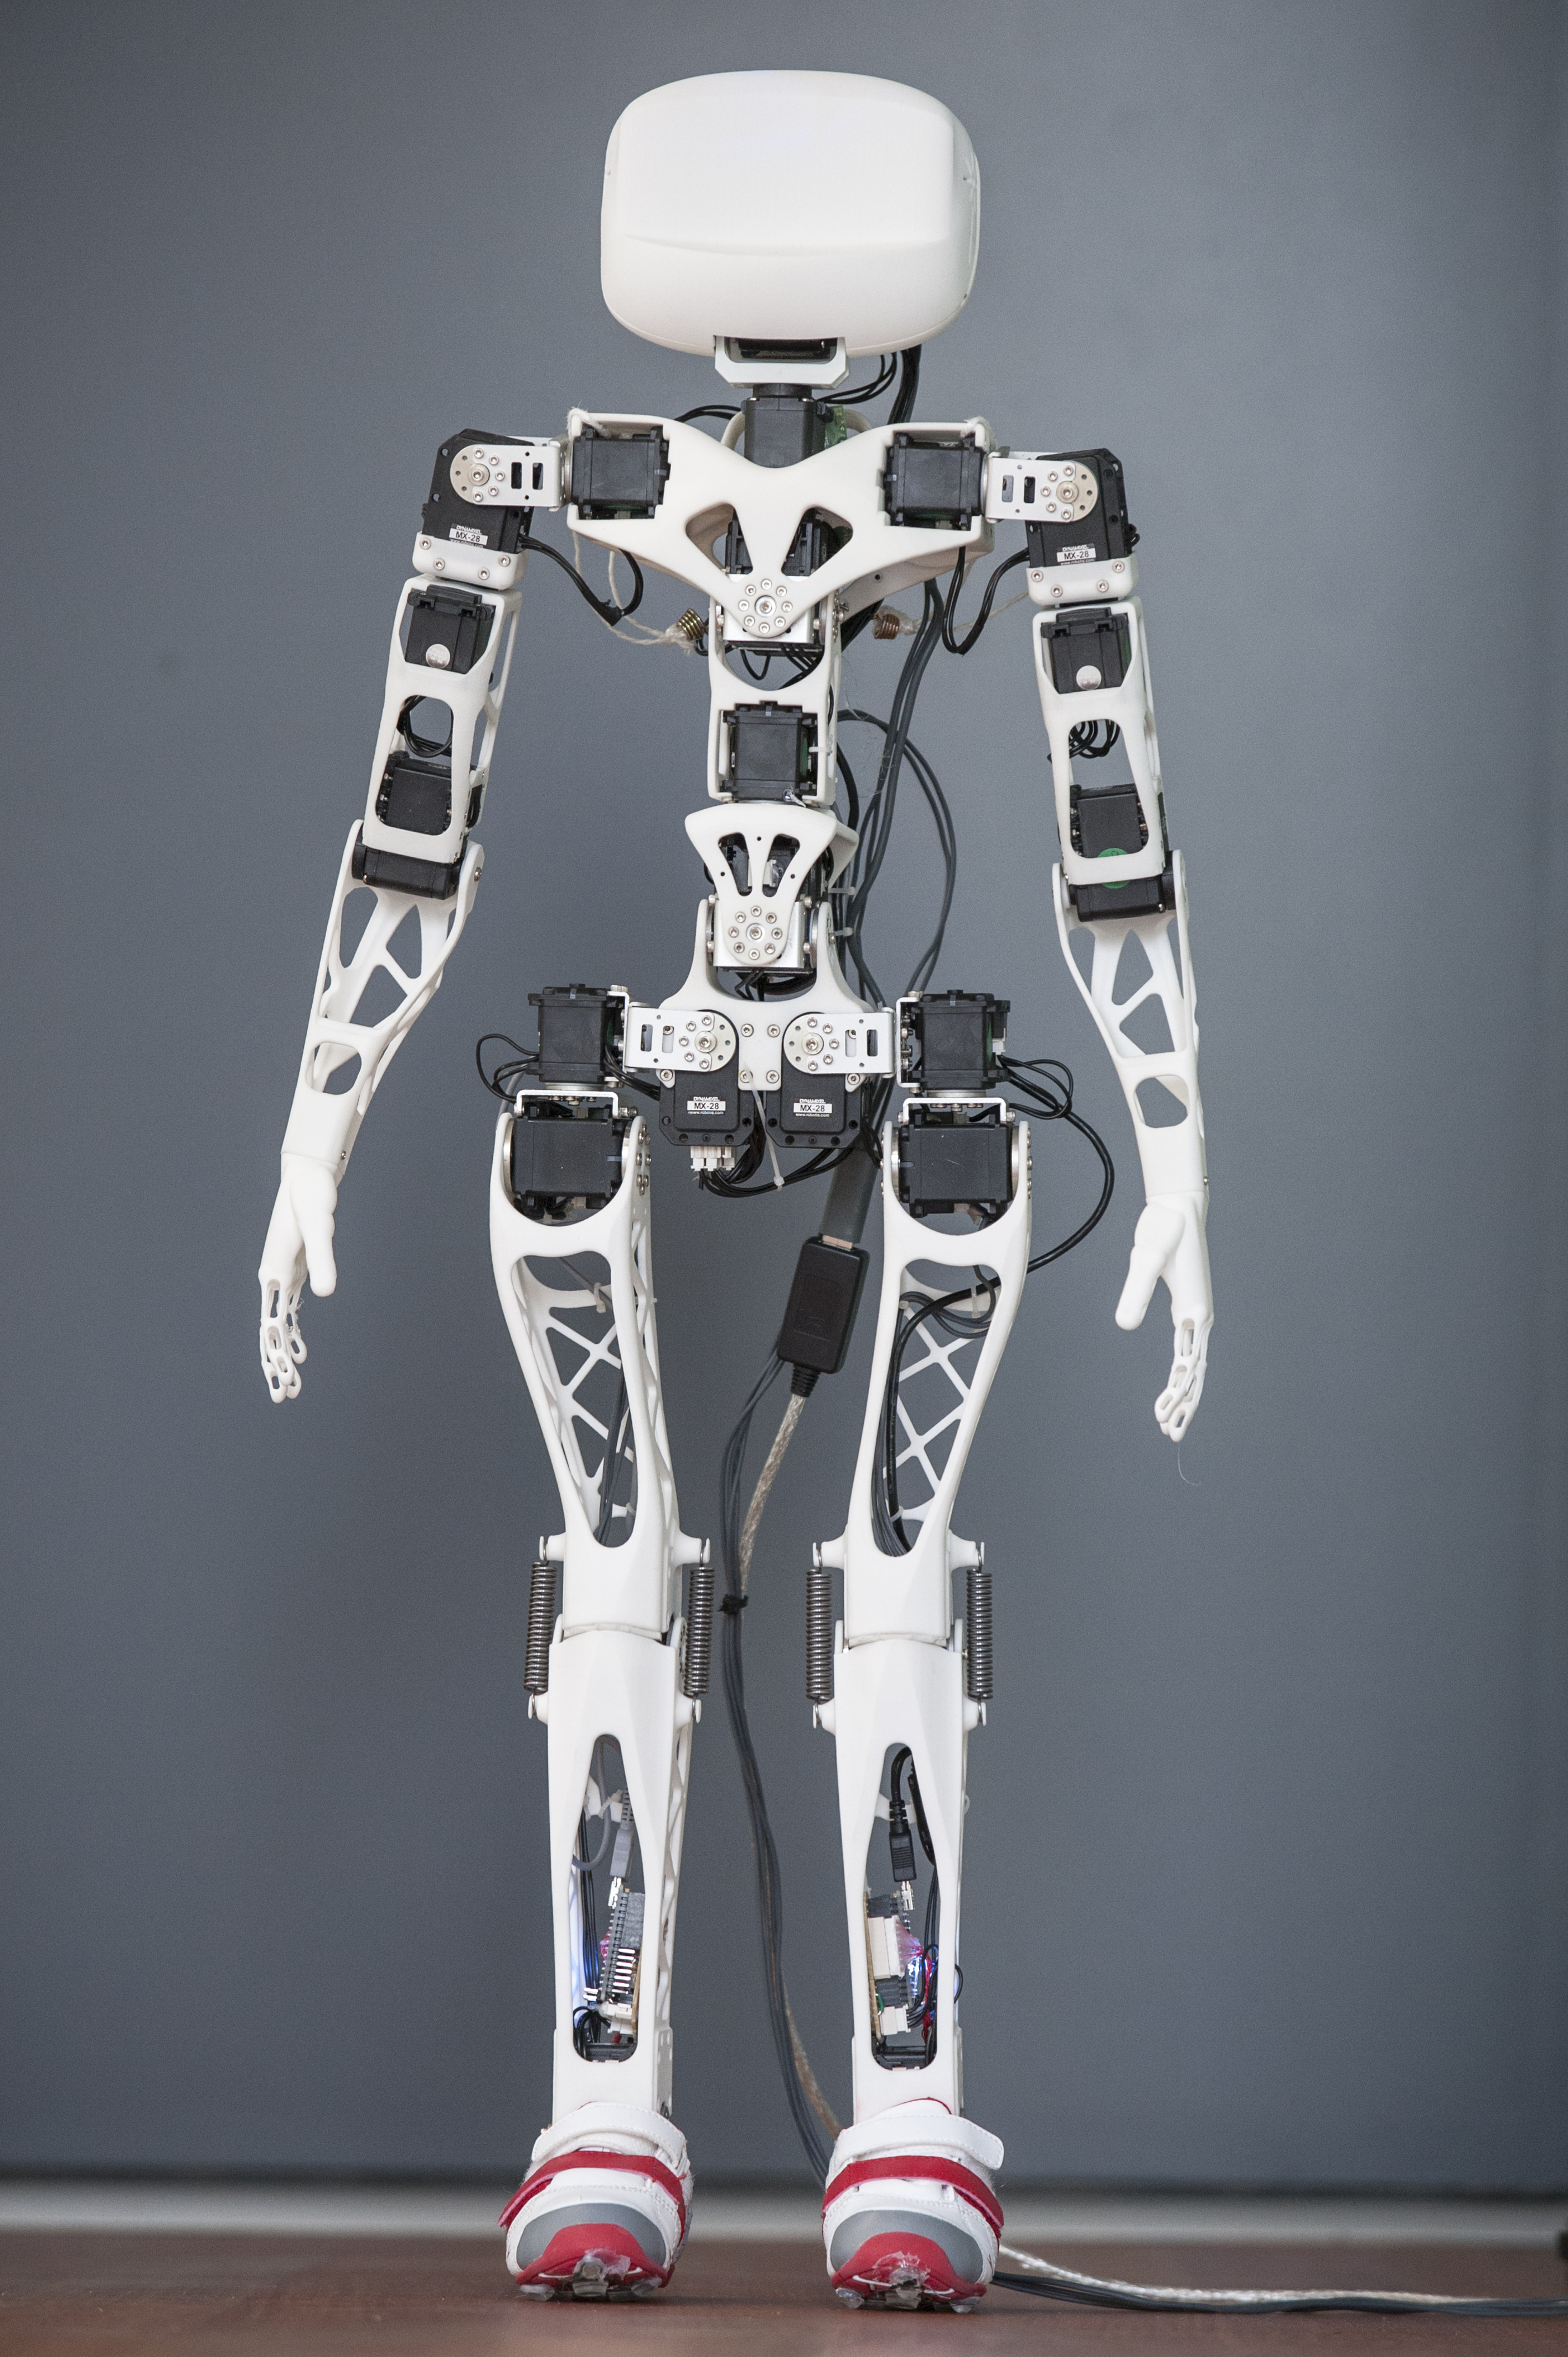
\includegraphics[width=0.3\linewidth]{presentation_images/17}
				\caption{Humanoid robot}
			\end{minipage}
		\end{figure}
	\end{frame}
	
%%%%%%%%%%%%%%%%%%%%%%%%%%%%%%%%%%%%%%%%%%%%%%%%%%%%%%%%%%%%%%%%%%%%%%%%%%%%%%%%%%%%%%%%%%%%%%%%%%%%%

	\begin{frame}
		\frametitle{Introduction and Motivation}
		\begin{block}{Why humanoids ?}
			\begin{itemize}
				\item
				Ability to work directly in the same human environment without any modification
				\item
				General-purpose workers
				\item
				Social integration
				\item
				Work with same tools as humans
			\end{itemize}
		\end{block}
	\end{frame}
	
%%%%%%%%%%%%%%%%%%%%%%%%%%%%%%%%%%%%%%%%%%%%%%%%%%%%%%%%%%%%%%%%%%%%%%%%%%%%%%%%%%%%%%%%%%%%%%%%%%%%%

\begin{frame}
	\frametitle{Introduction and Motivation}
	\begin{block}{Humanoids Advantages and Disadvantages}
		\begin{itemize}
			\item(+)
				Universal environment
			\item(+)
				Natural, human-like
			\item(+)
				Uneven terrains
			\item(-)
				Difficult locomotion
			\item(-)
				Complex design
			\item(-)
				Low speed
			\item(-)
				Complex control
			\item(?) Special tasks cannot be performed by general robots as good as by devices that were designed for this proper task.
		\end{itemize}
	\end{block}
\end{frame}

%%%%%%%%%%%%%%%%%%%%%%%%%%%%%%%%%%%%%%%%%%%%%%%%%%%%%%%%%%%%%%%%%%%%%%%%%%%%%%%%%%%%%%%%%%%%%%%%%%%%%

\begin{frame}
	\frametitle{Problem Overview}
	\begin{block}{Bipedal locomotion difficulties}
		\begin{itemize}
			\item
				Humanoids are underactuated due to inertia frame
			\item
				Difficult to solve Inverse Kinematics
			\item
				Several kinematic chains
			\item 
				Requires the robot to plan motions
		\end{itemize}
	\end{block}
	
	\begin{figure}[h!]
		\begin{minipage}[H]{\linewidth}
			\centering
			\includegraphics[scale=0.5]{presentation_images/7}
			\caption{Human as a kinematic chains, \cite{seo2011improved}}
		\end{minipage}
	\end{figure}
\end{frame}

%%%%%%%%%%%%%%%%%%%%%%%%%%%%%%%%%%%%%%%%%%%%%%%%%%%%%%%%%%%%%%%%%%%%%%%%%%%%%%%%%%%%%%%%%%%%%%%%%%%%%

	\begin{frame}
		\frametitle{Related work}
		\begin{block}{Bipedal locomotion control approaches}
			\begin{itemize}
				\item
					Analytical approach (ZMP based and others)
				\item
					Central Pattern Generator approach
				\item
					Neural Networks approach
				\item 
					Hidden Markov Model approach
				\item
					Rule based approach
			\end{itemize}
		\end{block}
	\end{frame}

%%%%%%%%%%%%%%%%%%%%%%%%%%%%%%%%%%%%%%%%%%%%%%%%%%%%%%%%%%%%%%%%%%%%%%%%%%%%%%%%%%%%%%%%%%%%%%%%%%%%%

	\begin{frame}
		\frametitle{Related work: Analytical approach}
		\begin{block}{Steps required for bipedal locomotion}
			\begin{itemize}
				\item
					Apply stability constraints
				\item
					Design a gait algorithm
				\item
					Solve remaining Degrees of Freedom
			\end{itemize}
		\end{block}
		\begin{block}{Stability measures}
			\begin{itemize}
				\item
					Zero Moment Point (ZMP)
				\item
					Foot Rotation Indicator (FRI)
			\end{itemize}
		\end{block}
	\end{frame}
	
%%%%%%%%%%%%%%%%%%%%%%%%%%%%%%%%%%%%%%%%%%%%%%%%%%%%%%%%%%%%%%%%%%%%%%%%%%%%%%%%%%%%%%%%%%%%%%%%%%%%%

	\begin{frame}
		\frametitle{Related work: Analytical approach}
		\begin{block}{ZMP}
			\begin{itemize}
				\item
					The distributed floor reaction force can be replaced by a single force R
acts on Zero Moment Point
			\end{itemize}
		\end{block}
		
		\begin{figure}[h!]
			\begin{minipage}[H]{\linewidth}
				\centering
				\includegraphics[width=0.5\linewidth]{presentation_images/8}
				\caption{Zero Moment Point (ZMP), \cite{vukobratovic2004zero}}
			\end{minipage}
		\end{figure}
	\end{frame}
	
%%%%%%%%%%%%%%%%%%%%%%%%%%%%%%%%%%%%%%%%%%%%%%%%%%%%%%%%%%%%%%%%%%%%%%%%%%%%%%%%%%%%%%%%%%%%%%%%%%%%%

	\begin{frame}
		\frametitle{Related work: Central Pattern Generator Approach}
		\begin{block}{Human walking process}
			\begin{itemize}
				\item
					Rhythm generating
				\item
					Control and adaptation mechanism
					
			\end{itemize}
		\end{block}
		\begin{block}{CPG principle}
			\begin{itemize}
				\item
					Biological CPGs are made from pairs of mutually inhibiting neurons
				\item
					Pairs of mutually inhibiting neurons are described by systems of differential equations
				\item
					CPG is a neural network working without input
			\end{itemize}
		\end{block}
	\end{frame}

%%%%%%%%%%%%%%%%%%%%%%%%%%%%%%%%%%%%%%%%%%%%%%%%%%%%%%%%%%%%%%%%%%%%%%%%%%%%%%%%%%%%%%%%%%%%%%%%%%%%%

	\begin{frame}
		\frametitle{Related work: Neural Networks Approach}
		\centering
		Feed-Forward Networks
		
		\begin{figure}[h!]
			\begin{minipage}[H]{\linewidth}
				\centering
				\includegraphics[width=\linewidth]{presentation_images/9}
				\caption{Feed Forward Network, \cite{kim2012zmp}}
			\end{minipage}
		\end{figure}
	\end{frame}

%%%%%%%%%%%%%%%%%%%%%%%%%%%%%%%%%%%%%%%%%%%%%%%%%%%%%%%%%%%%%%%%%%%%%%%%%%%%%%%%%%%%%%%%%%%%%%%%%%%%%

	\begin{frame}
		\frametitle{Related work: Neural Networks Approach}
		\centering
		Recurrent networks 
		
		\begin{figure}[h!]
			\begin{minipage}[H]{\linewidth}
				\centering
				\includegraphics[width=0.5\linewidth]{presentation_images/10}
				\caption{Elman Recurrent Network}
			\end{minipage}
		\end{figure}
	\end{frame}
	
%%%%%%%%%%%%%%%%%%%%%%%%%%%%%%%%%%%%%%%%%%%%%%%%%%%%%%%%%%%%%%%%%%%%%%%%%%%%%%%%%%%%%%%%%%%%%%%%%%%%%

	\begin{frame}
		\frametitle{Related work: Hidden Markov Model Approach}
		\begin{block}{HMM for bipedal locomotion algorithm}
			\begin{itemize}
				\item
					A correspondence between the control signal and controller input
				\item 
					 The control signal depends only on a finite number of previous input signals
				\item
					Define a set of patterns
				\item
					Set of input signals is mapped to the set of possible control signals
				\item
					Train the model by the data describing control signals
				\item
					 Collect a set of trained models
			\end{itemize}
		\end{block}
	\end{frame}
	
%%%%%%%%%%%%%%%%%%%%%%%%%%%%%%%%%%%%%%%%%%%%%%%%%%%%%%%%%%%%%%%%%%%%%%%%%%%%%%%%%%%%%%%%%%%%%%%%%%%%%

	\begin{frame}
		\frametitle{Related work: Rule Based Approach}
		\begin{block}{Rule Based Approach principle}
			\begin{itemize}
				\item
					Divide the set of all possible system configurations into the clusters
				\item 
					For each cluster assign the control function
				\item During the work control function will be chosen according to the current robot configuration
				\item
					Current configuration defines the possible control function
				\item Fuzzy logic controller is a perspective approach for solving dynamical stability problem
				\item Fuzzy logic controller divide all the configuration space into the subspaces
				\item For each subspace control function is defined in an optimal way
			\end{itemize}
		\end{block}
	\end{frame}

%%%%%%%%%%%%%%%%%%%%%%%%%%%%%%%%%%%%%%%%%%%%%%%%%%%%%%%%%%%%%%%%%%%%%%%%%%%%%%%%%%%%%%%%%%%%%%%%%%%%%

	\begin{frame}
		\frametitle{Theoretical aspects of bipedal robots control}
		\centering
		Locomotion is a periodic gait cycle.
		
		\begin{figure}[h!]
			\begin{minipage}[H]{\linewidth}
				\includegraphics[width=\linewidth]{presentation_images/26}
				\caption{Gait cycle decomposition, \cite{gait}}
			\end{minipage}
		\end{figure}
	\end{frame}
	
%%%%%%%%%%%%%%%%%%%%%%%%%%%%%%%%%%%%%%%%%%%%%%%%%%%%%%%%%%%%%%%%%%%%%%%%%%%%%%%%%%%%%%%%%%%%%%%%%%%%%

	\begin{frame}
		\frametitle{Theoretical aspects of bipedal robots control}
		\begin{block}{Cart table model}
			\begin{itemize}
				\item(+)
					Easy to understand
				\item(-)
					Is not precise
					
			\end{itemize}
		\end{block}
		
		\begin{figure}[h!]
			\begin{minipage}[H]{\linewidth}
				\centering
				\includegraphics[width=0.5\linewidth]{presentation_images/11}
				\caption{Cart table model, \cite{kajita2003biped}}
			\end{minipage}
		\end{figure}
	\end{frame}

%%%%%%%%%%%%%%%%%%%%%%%%%%%%%%%%%%%%%%%%%%%%%%%%%%%%%%%%%%%%%%%%%%%%%%%%%%%%%%%%%%%%%%%%%%%%%%%%%%%%%

	\begin{frame}
		\frametitle{Theoretical aspects of bipedal robots control: cart table model}
		\begin{equation}
			P = x - \dfrac{Z_c}{g} \ddot{x}
		\end{equation}		
		\begin{figure}[h!]
			\begin{minipage}[H]{\linewidth}
				\centering
				\includegraphics[width=0.4\linewidth]{presentation_images/11}
				\caption{Cart table model, \cite{kajita2003biped}}
			\end{minipage}
		\end{figure}
	\end{frame}

%%%%%%%%%%%%%%%%%%%%%%%%%%%%%%%%%%%%%%%%%%%%%%%%%%%%%%%%%%%%%%%%%%%%%%%%%%%%%%%%%%%%%%%%%%%%%%%%%%%%%

	\begin{frame}
		\frametitle{Theoretical aspects of bipedal robots control: cart table model}
		\begin{block}{Proper dynamics of cart table model}
			\begin{itemize}
				\item
					\begin{equation}
						\dfrac{d}{dt} \begin{bmatrix} x \\ \dot{x} \\ \ddot{x} \end{bmatrix} = \begin{bmatrix} 0 & 1 & 0 \\ 0 & 0 & 1 \\ 0 & 0& 0 \end{bmatrix}  \begin{bmatrix} x \\ \dot{x} \\ \ddot{x} \end{bmatrix} + \begin{bmatrix} 0 \\0 \\ 1 \end{bmatrix} u
					\end{equation}
				\item
					\begin{equation}
						p = \begin{bmatrix} 1 & 0  & - \dfrac{Z_c}{g} \end{bmatrix}\begin{bmatrix} x \\ \dot{x} \\ \ddot{x} \end{bmatrix}
					\end{equation}
				\item
					u is the third time derivative of x
			\end{itemize}
		\end{block}
	\end{frame}
	
%%%%%%%%%%%%%%%%%%%%%%%%%%%%%%%%%%%%%%%%%%%%%%%%%%%%%%%%%%%%%%%%%%%%%%%%%%%%%%%%%%%%%%%%%%%%%%%%%%%%%

	\begin{frame}
		\frametitle{Theoretical aspects of bipedal robots control}
		\begin{block}{Human planes intersting for locomotion}
			\begin{itemize}
				\item
					Sagittal plane
				\item
					Frontal plane
					
			\end{itemize}
		\end{block}
		
		\begin{figure}[h!]
			\begin{minipage}[H]{\linewidth}
				\centering
				\includegraphics[width=0.3\linewidth]{presentation_images/12}
				\caption{Human planes, \cite{medical}}
			\end{minipage}
		\end{figure}
	\end{frame}
	
%%%%%%%%%%%%%%%%%%%%%%%%%%%%%%%%%%%%%%%%%%%%%%%%%%%%%%%%%%%%%%%%%%%%%%%%%%%%%%%%%%%%%%%%%%%%%%%%%%%%%

	\begin{frame}
		\frametitle{Theoretical aspects of bipedal robots control}
		\begin{block}{Control principle}
			\begin{itemize}
				\item
				Find ZMP pattern that corresponds to wanted robot locomotion direction
				\item
				Calculate the cart trajectory to realize the given ZMP pattern
				\item
				Apply correction to robot in order to follow pattern
			\end{itemize}
		\end{block}
		
		\begin{figure}[h!]
			\begin{minipage}[H]{\linewidth}
				\centering
				\includegraphics[width=0.85\linewidth]{presentation_images/13}
				\caption{ZMP desired trajectory in frontal plane, \cite{kajita2003biped}}
			\end{minipage}
		\end{figure}
	\end{frame}
	
%%%%%%%%%%%%%%%%%%%%%%%%%%%%%%%%%%%%%%%%%%%%%%%%%%%%%%%%%%%%%%%%%%%%%%%%%%%%%%%%%%%%%%%%%%%%%%%%%%%%%

\begin{frame}
	\frametitle{Theoretical aspects of bipedal robots control}
	\begin{block}{Control principle}
		\begin{itemize}
			\item
			Find ZMP pattern that corresponds to wanted robot locomotion direction
			\item
			Calculate the cart trajectory to realize the given ZMP pattern
			\item
			Apply correction to robot in order to follow pattern
		\end{itemize}
	\end{block}
	
	\begin{figure}[h!]
		\begin{minipage}[H]{\linewidth}
			\centering
			\includegraphics[width=0.35\linewidth]{presentation_images/13}
		\end{minipage}
		\begin{minipage}[H]{\linewidth}
			\centering
			\includegraphics[width=0.35\linewidth]{presentation_images/14}
		\end{minipage}
		\caption{Inverse control principle, \cite{kajita2003biped}}
	\end{figure}
\end{frame}

%%%%%%%%%%%%%%%%%%%%%%%%%%%%%%%%%%%%%%%%%%%%%%%%%%%%%%%%%%%%%%%%%%%%%%%%%%%%%%%%%%%%%%%%%%%%%%%%%%%%%

	\begin{frame}
		\frametitle{Theoretical aspects of bipedal robots control}
		\begin{block}{Optimal Control}
			\begin{itemize}
				\item
					State space model
				\item
					Transfer function
				\item
					Transfer function measures
			\end{itemize}
		\end{block}
		
		\begin{figure}[h!]
			\includegraphics[width=0.5\linewidth]{presentation_images/15}
			\caption{Generalized regulator, \cite{hazell2008discrete}}
		\end{figure}
	\end{frame}

%%%%%%%%%%%%%%%%%%%%%%%%%%%%%%%%%%%%%%%%%%%%%%%%%%%%%%%%%%%%%%%%%%%%%%%%%%%%%%%%%%%%%%%%%%%%%%%%%%%%%

	\begin{frame}
		\frametitle{Theoretical aspects of bipedal robots control: Optimal Control}
		\begin{block}{Optimal Control}
			\begin{itemize}
				\item
					State space model
					\begin{equation}
						\begin{split}
							x(k+1) = Ax(k) + Bu(k)\\
							y(k) = Cx(k) + Du(k)
						\end{split}
					\end{equation}
				\item
					Transfer function
					\begin{equation}
						\begin{split}
							G(Z) = C(ZI - A)^{-1} B + D
						\end{split}
					\end{equation}
					
					Where Z is Z transform variable
			\end{itemize}
		\end{block}
	\end{frame}
	
%%%%%%%%%%%%%%%%%%%%%%%%%%%%%%%%%%%%%%%%%%%%%%%%%%%%%%%%%%%%%%%%%%%%%%%%%%%%%%%%%%%%%%%%%%%%%%%%%%%%%

\begin{frame}
	\frametitle{Theoretical aspects of bipedal robots control: Optimal Control}
	\begin{block}{Optimal Control}
		\begin{itemize}
			\item
				Transfer function measures
				
				\begin{equation}
					\begin{split}
						||G(Z)||_2 = Tr\{ B^{T} XB + D^{T} D \}
					\end{split}
				\end{equation}
			\item
				X should satisfy:
				\begin{equation}
					X = A^TXA + C^TC
				\end{equation}
			\item
				Physical meaning is a gain in power from input to output, assuming that the input signal is white noise.
		\end{itemize}
	\end{block}
\end{frame}

%%%%%%%%%%%%%%%%%%%%%%%%%%%%%%%%%%%%%%%%%%%%%%%%%%%%%%%%%%%%%%%%%%%%%%%%%%%%%%%%%%%%%%%%%%%%%%%%%%%%%

	\begin{frame}
		\frametitle{Theoretical aspects of bipedal robots control: Optimal Control}
		\begin{block}{Optimal Control}
			\begin{itemize}
				\item
					Transfer function measures
					
					\begin{equation}
						\begin{split}
							||G(Z)||_\infty = \sup_{\omega} \dfrac{||z||_2}{||\omega||_2}
						\end{split}
					\end{equation}
				\item
					\begin{equation}
					z  =G \omega
					\end{equation}
				\item
					$\omega$ is assumed to be a realization of a unit power, Gaussian, white noise
					process and z is the real values vector of input
				\item
					Physical meaning is a maximum possible gain in power from input to output, assuming that the input signal is white noise.
			\end{itemize}
		\end{block}
	\end{frame}

%%%%%%%%%%%%%%%%%%%%%%%%%%%%%%%%%%%%%%%%%%%%%%%%%%%%%%%%%%%%%%%%%%%%%%%%%%%%%%%%%%%%%%%%%%%%%%%%%%%%%

	\begin{frame}
		\frametitle{Theoretical aspects of bipedal robots control: Preview Control}
		\begin{block}{Preview Control}
			\begin{itemize}
				\item
					 Look forward for N discrete steps
				\item
					Predict the desirable value of controlled signal
				\item
					\cite{katayama1985design} proved the theorem that optimal control signal has the followong form:
					\begin{equation}
						u(k) = -G_I \sum^{k}_{i=0} e(i) - G_xx(k) - \sum^{N}_{l=1}G_d(l)y_d(k+l)
					\end{equation}
			\end{itemize}
		\end{block}
	\end{frame}
	
%%%%%%%%%%%%%%%%%%%%%%%%%%%%%%%%%%%%%%%%%%%%%%%%%%%%%%%%%%%%%%%%%%%%%%%%%%%%%%%%%%%%%%%%%%%%%%%%%%%%%

	\begin{frame}
		\frametitle{Theoretical aspects of bipedal robots control: Preview Control}
		It makes sense to find critical number of important future steps.
		\begin{figure}[h!]
			\begin{minipage}[H]{\linewidth}
				\centering
				\includegraphics[width=0.7\linewidth]{presentation_images/16}
				\caption{Preview Gain dependency from the time \cite{kajita2003biped}}
			\end{minipage}
		\end{figure}
	\end{frame}
	
%%%%%%%%%%%%%%%%%%%%%%%%%%%%%%%%%%%%%%%%%%%%%%%%%%%%%%%%%%%%%%%%%%%%%%%%%%%%%%%%%%%%%%%%%%%%%%%%%%%%%

	\begin{frame}
		\frametitle{Implementation and Evaluation}
		\begin{block}{What was done?}
			\begin{itemize}
				\item
					Implementation of cart table model
				\item
					Implementation of PID controlled cart table model
				\item
					Implementation of preview controlled cart table model
				\item
					Comparison of preview and PID control result
				\item
					Preview control was applied to robot model
			\end{itemize}
		\end{block}
	\end{frame}

%%%%%%%%%%%%%%%%%%%%%%%%%%%%%%%%%%%%%%%%%%%%%%%%%%%%%%%%%%%%%%%%%%%%%%%%%%%%%%%%%%%%%%%%%%%%%%%%%%%%%

\begin{frame}
	\frametitle{Implementation and Evaluation: }
	\begin{block}{Controller}
		\begin{itemize}
			\item
				PID controller
			\item
				Preview controller
		\end{itemize}
	\end{block}
	
	\begin{figure}[h!]
		\begin{minipage}[H]{\linewidth}
			\centering
			\includegraphics[width=0.35\linewidth]{presentation_images/13}
		\end{minipage}
		\begin{minipage}[H]{\linewidth}
			\centering
			\includegraphics[width=0.35\linewidth]{presentation_images/14}
		\end{minipage}
		\caption{Inverse control principle, \cite{kajita2003biped}}
	\end{figure}
\end{frame}

%%%%%%%%%%%%%%%%%%%%%%%%%%%%%%%%%%%%%%%%%%%%%%%%%%%%%%%%%%%%%%%%%%%%%%%%%%%%%%%%%%%%%%%%%%%%%%%%%%%%%

	\begin{frame}
		\frametitle{Summary}
		\begin{itemize}
			\item
				ololo
		\end{itemize}
	\end{frame}

%%%%%%%%%%%%%%%%%%%%%%%%%%%%%%%%%%%%%%%%%%%%%%%%%%%%%%%%%%%%%%%%%%%%%%%%%%%%%%%%%%%%%%%%%%%%%%%%%%%%%

	\begin{frame}
		\frametitle{Thanks for the attention}
		Now it's time for your questions
		\begin{figure}[h]
			%\center{\includegraphics[width=0.75\linewidth]{presentation_images/be_healthy.jpg}} 
		\end{figure}
	\end{frame}
	
%%%%%%%%%%%%%%%%%%%%%%%%%%%%%%%%%%%%%%%%%%%%%%%%%%%%%%%%%%%%%%%%%%%%%%%%%%%%%%%%%%%%%%%%%%%%%%%%%%%%%	
	\begin{frame}[allowframebreaks]
		\frametitle{Bibliography}    
			\bibliographystyle{apalike}
			\bibliography{robotics}
	\end{frame}
		
\end{document}
